%% 
%% Copyright 2007-2020 Elsevier Ltd
%% 
%% This file is part of the 'Elsarticle Bundle'.
%% ---------------------------------------------
%% 
%% It may be distributed under the conditions of the LaTeX Project Public
%% License, either version 1.2 of this license or (at your option) any
%% later version.  The latest version of this license is in
%%    http://www.latex-project.org/lppl.txt
%% and version 1.2 or later is part of all distributions of LaTeX
%% version 1999/12/01 or later.
%% 
%% The list of all files belonging to the 'Elsarticle Bundle' is
%% given in the file `manifest.txt'.
%% 
%% Template article for Elsevier's document class `elsarticle'
%% with harvard style bibliographic references

\documentclass[5p,times]{elsarticle}
%% Use the option review to obtain double line spacing
%% \documentclass[authoryear,preprint,review,12pt]{elsarticle}

%% Use the options 1p,twocolumn; 3p; 3p,twocolumn; 5p; or 5p,twocolumn
%% for a journal layout:
%% \documentclass[final,1p,times,authoryear]{elsarticle}
%% \documentclass[final,1p,times,twocolumn,authoryear]{elsarticle}
%% \documentclass[final,3p,times,authoryear]{elsarticle}
%% \documentclass[final,3p,times,twocolumn,authoryear]{elsarticle}
%% \documentclass[final,5p,times,authoryear]{elsarticle}
%% \documentclass[final,5p,times,twocolumn,authoryear]{elsarticle}

%% For including figures, graphicx.sty has been loaded in
%% elsarticle.cls. If you prefer to use the old commands
%% please give \usepackage{epsfig}

%% The amssymb package provides various useful mathematical symbols
\usepackage{amssymb}
%% The amsthm package provides extended theorem environments
%% \usepackage{amsthm}

%% The lineno packages adds line numbers. Start line numbering with
%% \begin{linenumbers}, end it with \end{linenumbers}. Or switch it on
%% for the whole article with \linenumbers.
%% \usepackage{lineno}

\usepackage[colorlinks=true, allcolors=blue]{hyperref}
\usepackage{booktabs,chemformula}
\usepackage{bbm}
\usepackage{algpseudocode}


\usepackage{hyperref}
\usepackage[acronym]{glossaries}

\hypersetup{%
  colorlinks=true,
  linkcolor=bluegray,
  citecolor=black,
  urlcolor=black,
  linktoc=all,
}

\renewcommand*{\glstextformat}[1]{\textcolor{black}{#1}}

\usepackage{makecell}


\makeglossaries
\loadglsentries{glossary}


% \theoremstyle{definition}
\newtheorem{definition}{Definition}[section]

\journal{Nuclear Physics B}

\begin{document}

\begin{frontmatter}

%% Title, authors and addresses

%% use the tnoteref command within \title for footnotes;
%% use the tnotetext command for theassociated footnote;
%% use the fnref command within \author or \affiliation for footnotes;
%% use the fntext command for theassociated footnote;
%% use the corref command within \author for corresponding author footnotes;
%% use the cortext command for theassociated footnote;
%% use the ead command for the email address,
%% and the form \ead[url] for the home page:
%% \title{Title\tnoteref{label1}}
%% \tnotetext[label1]{}
%% \author{Name\corref{cor1}\fnref{label2}}
%% \ead{email address}
%% \ead[url]{home page}
%% \fntext[label2]{}
%% \cortext[cor1]{}
%% \affiliation{organization={},
%%            addressline={}, 
%%            city={},
%%            postcode={}, 
%%            state={},
%%            country={}}
%% \fntext[label3]{}


% \title{Towards Explainable Time-Series Extrinsic Regression for Biological Age Estimation}
\title{How to improve your health by changing your habits?}

%% use optional labels to link authors explicitly to addresses:
%% \author[label1,label2]{}
%% \affiliation[label1]{organization={},
%%             addressline={},
%%             city={},
%%             postcode={},
%%             state={},
%%             country={}}
%%
%% \affiliation[label2]{organization={},
%%             addressline={},
%%             city={},
%%             postcode={},
%%             state={},
%%             country={}}
% Julia E. Vogt
% View ORCID ID profile
% Department of Computer Science, ETH Zurich, Universitätstrasse 6, 8092, Zürich, Switzerland

\author[inst1]{Alexis Tabin}
\author[inst1]{Patrick Langer}
\author[inst2]{Julia E. Vogt}

\affiliation[inst1]{organization={Department of Management, Technology, and Economics},%Department and Organization
            addressline={Weinbergstrasse 56/58}, 
            city={ETH Zurich},
            state={Zurich},
            country={Switzerland}}
\affiliation[inst2]{organization={Department of Computer Science},%Department and Organization
            addressline={Universitatstrasse 6}, 
            city={ETH Zurich},
            state={Zurich},
            country={Switzerland}}



\begin{abstract}
Noninvasive, smart, and wearable devices such as smartphones and smartwatches collect a vast amount of multimodal data that potentially contains valuable information about our daily activities and habits.
% 
Machine learning can aggregate these data to create digital biomarkers. The latter can potentially enable personalized and timely interventions to detect and prevent chronic diseases at an early stage. However, current digital biomarkers cannot prevent diseases before they occur because they are currently unable to assess a person's general health state. 
% 
By leveraging advancements in digital health, we investigate the utility of generating recommendations to improve a person's general health state based on physical activity data. The biological age predicted from the physical activity data using deep learning models as a proxy is used to assess a person's health state.
% 
To generate recommendations using the deep learning models, four novel counterfactual algorithms for time series extrinsic regression tasks derived from prior work on time series classification are introduced. Furthermore, we conducted qualitative and quantitative analyses of their performances and obtained indicative health recommendations that patients could use to improve their daily habits.
\end{abstract}

% %%Graphical abstract
% \begin{graphicalabstract}
% 
\includegraphics{grabs}
% \end{graphicalabstract}

% %%Research highlights
% \begin{highlights}
% \item Research highlight 1
% \item Research highlight 2
% \end{highlights}

\begin{keyword}
%% keywords here, in the form: keyword \sep keyword
Deep Learning \sep Time Series \sep Extrinsic Regression \sep Counterfactuals \sep Explanations%% PACS codes here, in the form: \PACS code \sep code
% \PACS 0000 \sep 1111
%% MSC codes here, in the form: \MSC code \sep code
%% or \MSC[2008] code \sep code (2000 is the default)
% \MSC 0000 \sep 1111
\end{keyword}

\end{frontmatter}

%% \linenumbers

%% main text

\section{Introduction}
\label{sec:introduction}

% \textbf{Health related aspects}
% Healthcare costs are exploding
% Monitoring health variables on a regular basis can help prevent chronic diseases rather than just reacting to them after they have developed.

% \textbf{Deep Learning can infer Biological Age from Physical Activity}
% AI can be used to monitor health simply through PA
% But AI cannot tell how to change.

% \textbf{Goal of the paper}
% Explain what the patient should do to improve his health. 
% Show that there is a gap in the research and that it is very much needed in healthcare.


%============ Written by ChatGPT ============
In contemporary healthcare landscapes, the challenge of escalating healthcare costs looms large. Amidst this backdrop, the imperative of shifting from reactive to proactive healthcare strategies gains prominence. One promising avenue is the utilization of deep learning methodologies to glean insights from an individual's \acrfull{pa} data, thereby inferring crucial health indicators such as biological age. However, while the potential of \acrfull{ai} in health monitoring is vast, a critical gap persists: the translation of \acrshort{ai}-derived insights into actionable steps for individuals to improve their health.\\

\textbf{Health Related Aspects} Healthcare costs continue to spiral upward, underscoring the urgency of preventative healthcare measures. Monitoring health variables regularly presents a proactive approach to mitigating the onset of chronic diseases, contrasting with the traditional reactive model of healthcare intervention. Moreover, the burden of chronic diseases on both individuals and healthcare systems necessitates a paradigm shift towards proactive measures aimed at early detection and prevention.\\

\textbf{Deep Learning Can Infer Biological Age from Physical Activity} The advent of deep learning algorithms has facilitated the extraction of nuanced health information from \acrshort{pa} data alone. Yet, while \acrshort{ai} can proficiently analyze and infer biological age, it currently falls short in providing personalized guidance on how individuals can effectuate tangible changes in their lifestyle to enhance their health outcomes.\\

\textbf{Goal of the Paper} This paper endeavours to bridge this crucial gap by elucidating actionable steps individuals can undertake to ameliorate their health trajectory based on insights derived from \acrshort{ai}-driven analysis of their physical activity data. By demonstrating the dearth of research addressing this vital translation step, we underscore the pressing need for such interventions within the healthcare domain.

In the ensuing sections, we delve into the methodologies employed for inferring biological age from physical activity data and subsequently propose a framework for translating these insights into personalized health recommendations. Through this exploration, we aim to underscore the transformative potential of integrating \acrshort{ai}-driven health monitoring with actionable guidance, thereby revolutionizing preventative healthcare practices.
%============ Written by ChatGPT ============

\section{Related Work}
\label{sec:related-work}
% \textbf{Explainable Artificial Intelligence on Time-Series Data} An Overview of existing Explainable Artificial Intelligence (XAI) on Time-Series Data shows that the main focus is on the classification task.

% We are interested in post-hoc explainability methods, with a preference for model-agnostic types. Post-hoc methods refer to the fact that the explainability module wraps the model to produce an explanation. On the other hand, ante-hoc methods incorporate the explainability module into the model's architecture. The agnostic type refers to the fact that the explainability methods do not depend on the model and should work with any type of model. 

% The scope of the explanation can be either local or global. The local scope would mean that the methods could explain which behaviours for the patient are good or bad. General scope tends to identify good or bad behaviour in the whole population.

% The target of the explanation is the patient himself.

% And the problem type should be extrinsic regression.
% 
\begin{table*}[h!]
  \centering
  \begin{tabular}{@{}ccccccccccc@{}}
    \toprule
    Date        &   Authors                         & Model             & Methods       & Spec./Agno.   & Scope         & Target  & Problem Type                      & Citations         & Code \\
    \midrule

    2013        & Senin\cite{senin_sax-vsm_2013}             &\textit{Sax-vsm}   & SAX           & Specific      & Global        & Dev.      & Classification                    & 379               & \href{https://github.com/jMotif/sax-vsm_classic}{code}\\ 
    
    2016        &   Wang \cite{wang_time_2016}        & \textit{FCN}      & Backprop.     & Specific      & Local         & Dev.      & Classification                    & 1688              & \href{https://github.com/cauchyturing/UCR_Time_Series_Classification_Deep_Learning_Baseline}{code}\\ 

    2017        & Karim\cite{karim_multivariate_2019}             &\textit{\footnotesize{LSTM-FCN}} & Attention     &Specific       & Local         & Dev.      & Classification                    & 1143              & \href{https://github.com/houshd/LSTM-FCN}{code}\\ 

    2018        & Wachter\cite{wachter_counterfactual_2018} & \textit{W-CF} & CF    & Agnostic      & Local         & User      & Classification & 2584 & \href{https://github.com/e-delaney/Instance-Based_CFE_TSC/tree/main/W-CF}{code}\\

    2018        & Vinayavekhin\cite{vinayavekhin_focusing_2018} &\textit{TCL}& Attention &Specific        & Local         & Dev.      & Class. \& Fore.                           & 25                & no\\  

    2018        & Strodthoff\cite{strodthoff_detecting_2019}  &\textit{\footnotesize{MI-FCNN}}   & Backprop.     &Specific       & Local         & User   & Classification                    & 176               & no\\ 

    2018        & Siddiqui\cite{siddiqui_tsviz_2019}       &\textit{Tsviz}     & Backprop.     &Specific       & Both          & Dev.      & Class. \& Reg.                    & 78                & \href{https://github.com/shoaibahmed/TSViz-Core}{code}\\

    2018        & Le Nguyen\cite{nguyen_interpretable_2018}&\textit{SEQL}&SAX        &Specific       & Global        & Dev.      & Classification                    & 11                & \href{https://github.com/lnthach/Mr-SEQL}{code}\\ 

    2018        & Cho\cite{cho_interpretation_2020}   &\textit{CHAP}      & Backprop.     & Specific      & Both          & Dev.      & Classification                           & 176               & no\\

    2018        & Ge\cite{ge_interpretable_2018}      &\textit{\footnotesize{ICU-LSTM}}  & Attention     &Specific       & Global        & Dev.      & Prediction                        & 68                & no \\  

    2018        & El-Sappagh\cite{el-sappagh_ontology-based_2018}   & \textit{FAHP}     & Fuzy logic    &Specific       & Global        & User      & Classification                    & 78                & no\\ 

    2019        &   Fawaz \cite{ismail_fawaz_accurate_2019}  & \textit{\footnotesize{ESS-CNN}}  & Backprop.     &Specific       & Local         & User   & Class. \& Reg.                    & 86                & \href{https://github.com/hfawaz/ijcars19}{code}\\ 

    2019        &  Wang\cite{wang_learning_2019}      &\textit{PR-CNN} & Sapelets      &Specific       & Global        & Dev.      & Classification                    & 17                & no\\ 

    2019        &   Oviedo \cite{oviedo_fast_2019}    & \textit{AutoXRD}  & Backprop.     &Specific       & Both          & Dev.      & Classification                    & 198               & \href{https://github.com/PV-Lab/autoXRD/tree/master}{code}\\ 

    2019        & Kashiparekh\cite{kashiparekh_convtimenet_2019}&\textit{ConvNet}& Perturbation  &Agnostic       & Local         & Dev.      & Classification                    & 89                & no \\ 

    2019        & Choi\cite{choi_fully_2021}               &\textit{IDH}& Attention   &Specific       & Local         & Dev.      & Classification                                 & 92                & \href{https://github.com/yoonchoi-neuro/automated_hybrid_IDH}{code}\\  

    2019        & Tonekaboni\cite{tonekaboni_explaining_2019}&\textit{FFC}& CF&Agnostic    & Both          & Dev.      & Classification                           & 8                & no \\ 

    2019        & Assaf\cite{assaf_mtex-cnn_2019}                  &\textit{Mtex-cnn}  & Backprop.&Specific       & Local         & Dev.      & Forecasting                        & 51                & no\\ 

    2019        & Munir\cite{munir_tsxplain_2019}            &\textit{Tsxplain}  &  Backprop.    &Agnostic       & Local         & Dev.      & Classification                    & 17                & no\\  

    2019        & Gee\cite{gee_explaining_2019}        &\textit{PDL}       & Prototypes    &Specific       & Global        & Dev.      & Classification                    & 66                & \href{https://github.com/alangee/ijcai19-ts-prototypes}{code} \\ 

    2020        & Li\cite{li_efficient_2022}                   &\textit{\footnotesize{BSPCOVER}}  & Shapelets     & Specific      & Global        & Dev.      & Classification                    & 43               & no\\  

    2020        & Augustin\cite{augustin_adversarial_2020}&\textit{RATIO} & CF&Agnostic      & Local         & Dev.      & Training                          & 70                & \href{https://github.com/M4xim4l/InNOutRobustness}{code}\\ 
    
    2020        & Hao\cite{hao_new_2020}                 &\textit{CA-SFCN}   & Attention     &Specific       & Local         & Dev.      & Classification                    & 30                & \href{https://github.com/huipingcao/nmsu_yhao_ijcai2020}{code}\\ 

    2020        &   Wolanin\cite{wolanin_estimating_2020}       & \textit{CY-EDL}   & Backprop.     &Specific       & Both          & User   & Forecasting                          & 125               & no \\

    2020        & Kidger\cite{kidger_generalised_2020}& \textit{GST}      & Shapelets     &Specific       & Global        & Dev.      & Classification                    & 9                 & \href{https://github.com/patrick-kidger/generalised_shapelets}{code}\\  

    2020        & Schockaert\cite{schockaert_attention_2020} & \textit{\footnotesize{AM-LSTM}}& Attention&Specific       & Both          & Dev.      & Forecasting                       & 6                 & no\\ 

    2020        & Siddiqui\cite{siddiqui_tsinsight_2020}& \textit{Tsinsight}& Attention   &Specific       &Both           & Dev.      & Classification                    & 12                & no \\ 

    2020        & Tan\cite{tan_explainable_2021}                 &\textit{\footnotesize{eUA-CRNN}}  & Attention     &Specific       & Local         & Dev.      & Classification                                & 28                & no\\  

    2020        & Pan\cite{pan_series_2020}           &\textit{Saliency}& Perturbation    &Agnostic       & Local         & Dev.      & Forecasting                       & 7                 & no \\ 

    2020        & Ismail\cite{ismail_benchmarking_2020}           &\textit{Saliency}& Perturbation    &Agnostic       & Local         & Dev.      & Classification                    & 124               & \href{https://github.com/ayaabdelsalam91/TS-Interpretability-Benchmark}{code}\\ 

    2020        & Wang\cite{wang_deep_2021}           & \textit{\footnotesize{Deep-FCM}}& Fuzzy logic    &Specific       & Global        & Dev.      & Prediction                        & 39                & no\\ 

    2020        & Lauristsen\cite{lauritsen_early_2020}   &\textit{TCN}       &Backprop.      &Specific       & Both          & Dev.      & Classification                    & 234               & \href{https://github.com/albermax/innvestigate}{1} and \href{https://github.com/slundberg/shap}{2} \\

    2021        &Crabbé\cite{crabbe_explaining_2021}    & \textit{DynaMask}     & Perturbation  & Agnostic      & Local     & Dev.      & Class. \& Reg.                    & 55            & \href{https://github.com/JonathanCrabbe/Dynamask}{code}   \\ 

    2021        & Lim\cite{lim_temporal_2020}         & \textit{TFT}      & Attention     &Specific       & Both          & Dev.      & Forecasting                       & 822               & \href{https://github.com/greatwhiz/tft_tf2}{code}       \\ 

    2021        & Delaney\cite{delaney_instance-based_2021} & \textit{\footnotesize{Native Guide}} & CF & Agnostic & Local & Both      & Classification & 92 & \href{https://github.com/e-delaney/Instance-Based_CFE_TSC/tree/main}{code} \\
  
    2022        &Gao\cite{gao_explainable_2022}       &  \textit{ETNODE}  & Attention     &Specific       & Both          & Dev.      & Forecasting                        & 8                 & \href{https://github.com/PengleiGao/ETN-ODE}{code} \\  

    2023        &Zhao\cite{zhao_explainable_2023}                &\textit{Att-TCN}   & Perturbation             & Agnostic             & Both             & Dev.          & Classification                    & 3                 & no \\ 

    2023        & Höllig\cite{hollig_tsevo_2022}           & \textit{TSEvo}& CF           & Agnostic             & Local             & User         & Classification                                 & 5                 & \href{https://github.com/fzi-forschungszentrum-informatik/TSInterpret}{code} \\

    2024        & Ours           & \textit{TSEvoR}& CF           & Agnostic             & Local             & User         & Regression                   & -                 & \href{https://github.com/AlexisTabin/BA-Estimation-TCN}{code} \\

    \bottomrule
  \end{tabular}
  \caption{Comparison of the existing XAI techniques for Time-Series, adapted from \cite{rojat_explainable_2021}}
\end{table*}

% \textbf{Counterfactuals Explanations for Time-Series Classification} Counterfactuals are very close to Adversarial Perturbations \cite{moosavi-dezfooli_universal_2017}. The main difference between them is the sparsity factor. Adversarial Perturbations are used mainly when handling image classification. The goal is to show that a very similar image could be classified differently with changes in the input that are unnoticeable by the human eye. To achieve that, the Adversarial Perturbation model modifies many variables by a small value, whereas the Counterfactuals want to modify the least number possible of variables to achieve human interpretable solutions. Wachter \& Al. \cite{wachter_counterfactual_2018} were among the first to propose a Counterfactual theory. 
% Definition of Counterfactuals, Wachter equation 

% \textbf{GAP - From Counterfactuals for Time-Series Classification to Counterfactuals for Time-Series Extrinsic Regression}
% Explain existing techniques

%============ Written by ChatGPT ============
\subsection{Explainable Artificial Intelligence on Time-Series Data} Existing research on Explainable Artificial Intelligence (XAI) for time-series data predominantly focuses on classification tasks. \\
Here, the emphasis will be put on post-hoc explainability methods, specifically prioritizing techniques that work across different types of models, known as model-agnostic approaches.
Post-hoc methods wrap an explainability module around the model to generate explanations, contrasting with ante-hoc methods that integrate explainability within the model's architecture.
Model-agnostic methods are preferred due to their versatility across various model types. \\
Additionally, explainability scopes vary, encompassing both local and global perspectives.
Local explanations provide insights into individual behaviours, while global explanations discern broader trends within populations.
Crucially, the patients themselves are the target audience for explanations, aligning with the overarching goal of personalized healthcare interventions.\\
Furthermore, the problem type addressed typically falls under the name of time-series extrinsic regression, where the goal is to learn a relationship between a time-serie and a continuous scalar variable \cite{tan_time_2021}.


\begin{table*}[h!]
  \centering
  \begin{tabular}{@{}ccccccccccc@{}}
    \toprule
    Date        &   Authors                         & Model             & Methods       & Spec./Agno.   & Scope         & Target  & Problem Type                      & Citations         & Code \\
    \midrule

    2013        & Senin\cite{senin_sax-vsm_2013}             &\textit{Sax-vsm}   & SAX           & Specific      & Global        & Dev.      & Classification                    & 379               & \href{https://github.com/jMotif/sax-vsm_classic}{code}\\ 
    
    2016        &   Wang \cite{wang_time_2016}        & \textit{FCN}      & Backprop.     & Specific      & Local         & Dev.      & Classification                    & 1688              & \href{https://github.com/cauchyturing/UCR_Time_Series_Classification_Deep_Learning_Baseline}{code}\\ 

    2017        & Karim\cite{karim_multivariate_2019}             &\textit{\footnotesize{LSTM-FCN}} & Attention     &Specific       & Local         & Dev.      & Classification                    & 1143              & \href{https://github.com/houshd/LSTM-FCN}{code}\\ 

    2018        & Wachter\cite{wachter_counterfactual_2018} & \textit{W-CF} & CF    & Agnostic      & Local         & User      & Classification & 2584 & \href{https://github.com/e-delaney/Instance-Based_CFE_TSC/tree/main/W-CF}{code}\\

    2018        & Vinayavekhin\cite{vinayavekhin_focusing_2018} &\textit{TCL}& Attention &Specific        & Local         & Dev.      & Class. \& Fore.                           & 25                & no\\  

    2018        & Strodthoff\cite{strodthoff_detecting_2019}  &\textit{\footnotesize{MI-FCNN}}   & Backprop.     &Specific       & Local         & User   & Classification                    & 176               & no\\ 

    2018        & Siddiqui\cite{siddiqui_tsviz_2019}       &\textit{Tsviz}     & Backprop.     &Specific       & Both          & Dev.      & Class. \& Reg.                    & 78                & \href{https://github.com/shoaibahmed/TSViz-Core}{code}\\

    2018        & Le Nguyen\cite{nguyen_interpretable_2018}&\textit{SEQL}&SAX        &Specific       & Global        & Dev.      & Classification                    & 11                & \href{https://github.com/lnthach/Mr-SEQL}{code}\\ 

    2018        & Cho\cite{cho_interpretation_2020}   &\textit{CHAP}      & Backprop.     & Specific      & Both          & Dev.      & Classification                           & 176               & no\\

    2018        & Ge\cite{ge_interpretable_2018}      &\textit{\footnotesize{ICU-LSTM}}  & Attention     &Specific       & Global        & Dev.      & Prediction                        & 68                & no \\  

    2018        & El-Sappagh\cite{el-sappagh_ontology-based_2018}   & \textit{FAHP}     & Fuzy logic    &Specific       & Global        & User      & Classification                    & 78                & no\\ 

    2019        &   Fawaz \cite{ismail_fawaz_accurate_2019}  & \textit{\footnotesize{ESS-CNN}}  & Backprop.     &Specific       & Local         & User   & Class. \& Reg.                    & 86                & \href{https://github.com/hfawaz/ijcars19}{code}\\ 

    2019        &  Wang\cite{wang_learning_2019}      &\textit{PR-CNN} & Sapelets      &Specific       & Global        & Dev.      & Classification                    & 17                & no\\ 

    2019        &   Oviedo \cite{oviedo_fast_2019}    & \textit{AutoXRD}  & Backprop.     &Specific       & Both          & Dev.      & Classification                    & 198               & \href{https://github.com/PV-Lab/autoXRD/tree/master}{code}\\ 

    2019        & Kashiparekh\cite{kashiparekh_convtimenet_2019}&\textit{ConvNet}& Perturbation  &Agnostic       & Local         & Dev.      & Classification                    & 89                & no \\ 

    2019        & Choi\cite{choi_fully_2021}               &\textit{IDH}& Attention   &Specific       & Local         & Dev.      & Classification                                 & 92                & \href{https://github.com/yoonchoi-neuro/automated_hybrid_IDH}{code}\\  

    2019        & Tonekaboni\cite{tonekaboni_explaining_2019}&\textit{FFC}& CF&Agnostic    & Both          & Dev.      & Classification                           & 8                & no \\ 

    2019        & Assaf\cite{assaf_mtex-cnn_2019}                  &\textit{Mtex-cnn}  & Backprop.&Specific       & Local         & Dev.      & Forecasting                        & 51                & no\\ 

    2019        & Munir\cite{munir_tsxplain_2019}            &\textit{Tsxplain}  &  Backprop.    &Agnostic       & Local         & Dev.      & Classification                    & 17                & no\\  

    2019        & Gee\cite{gee_explaining_2019}        &\textit{PDL}       & Prototypes    &Specific       & Global        & Dev.      & Classification                    & 66                & \href{https://github.com/alangee/ijcai19-ts-prototypes}{code} \\ 

    2020        & Li\cite{li_efficient_2022}                   &\textit{\footnotesize{BSPCOVER}}  & Shapelets     & Specific      & Global        & Dev.      & Classification                    & 43               & no\\  

    2020        & Augustin\cite{augustin_adversarial_2020}&\textit{RATIO} & CF&Agnostic      & Local         & Dev.      & Training                          & 70                & \href{https://github.com/M4xim4l/InNOutRobustness}{code}\\ 
    
    2020        & Hao\cite{hao_new_2020}                 &\textit{CA-SFCN}   & Attention     &Specific       & Local         & Dev.      & Classification                    & 30                & \href{https://github.com/huipingcao/nmsu_yhao_ijcai2020}{code}\\ 

    2020        &   Wolanin\cite{wolanin_estimating_2020}       & \textit{CY-EDL}   & Backprop.     &Specific       & Both          & User   & Forecasting                          & 125               & no \\

    2020        & Kidger\cite{kidger_generalised_2020}& \textit{GST}      & Shapelets     &Specific       & Global        & Dev.      & Classification                    & 9                 & \href{https://github.com/patrick-kidger/generalised_shapelets}{code}\\  

    2020        & Schockaert\cite{schockaert_attention_2020} & \textit{\footnotesize{AM-LSTM}}& Attention&Specific       & Both          & Dev.      & Forecasting                       & 6                 & no\\ 

    2020        & Siddiqui\cite{siddiqui_tsinsight_2020}& \textit{Tsinsight}& Attention   &Specific       &Both           & Dev.      & Classification                    & 12                & no \\ 

    2020        & Tan\cite{tan_explainable_2021}                 &\textit{\footnotesize{eUA-CRNN}}  & Attention     &Specific       & Local         & Dev.      & Classification                                & 28                & no\\  

    2020        & Pan\cite{pan_series_2020}           &\textit{Saliency}& Perturbation    &Agnostic       & Local         & Dev.      & Forecasting                       & 7                 & no \\ 

    2020        & Ismail\cite{ismail_benchmarking_2020}           &\textit{Saliency}& Perturbation    &Agnostic       & Local         & Dev.      & Classification                    & 124               & \href{https://github.com/ayaabdelsalam91/TS-Interpretability-Benchmark}{code}\\ 

    2020        & Wang\cite{wang_deep_2021}           & \textit{\footnotesize{Deep-FCM}}& Fuzzy logic    &Specific       & Global        & Dev.      & Prediction                        & 39                & no\\ 

    2020        & Lauristsen\cite{lauritsen_early_2020}   &\textit{TCN}       &Backprop.      &Specific       & Both          & Dev.      & Classification                    & 234               & \href{https://github.com/albermax/innvestigate}{1} and \href{https://github.com/slundberg/shap}{2} \\

    2021        &Crabbé\cite{crabbe_explaining_2021}    & \textit{DynaMask}     & Perturbation  & Agnostic      & Local     & Dev.      & Class. \& Reg.                    & 55            & \href{https://github.com/JonathanCrabbe/Dynamask}{code}   \\ 

    2021        & Lim\cite{lim_temporal_2020}         & \textit{TFT}      & Attention     &Specific       & Both          & Dev.      & Forecasting                       & 822               & \href{https://github.com/greatwhiz/tft_tf2}{code}       \\ 

    2021        & Delaney\cite{delaney_instance-based_2021} & \textit{\footnotesize{Native Guide}} & CF & Agnostic & Local & Both      & Classification & 92 & \href{https://github.com/e-delaney/Instance-Based_CFE_TSC/tree/main}{code} \\
  
    2022        &Gao\cite{gao_explainable_2022}       &  \textit{ETNODE}  & Attention     &Specific       & Both          & Dev.      & Forecasting                        & 8                 & \href{https://github.com/PengleiGao/ETN-ODE}{code} \\  

    2023        &Zhao\cite{zhao_explainable_2023}                &\textit{Att-TCN}   & Perturbation             & Agnostic             & Both             & Dev.          & Classification                    & 3                 & no \\ 

    2023        & Höllig\cite{hollig_tsevo_2022}           & \textit{TSEvo}& CF           & Agnostic             & Local             & User         & Classification                                 & 5                 & \href{https://github.com/fzi-forschungszentrum-informatik/TSInterpret}{code} \\

    2024        & Ours           & \textit{TSEvoR}& CF           & Agnostic             & Local             & User         & Regression                   & -                 & \href{https://github.com/AlexisTabin/BA-Estimation-TCN}{code} \\

    \bottomrule
  \end{tabular}
  \caption{Comparison of the existing XAI techniques for Time-Series, adapted from \cite{rojat_explainable_2021}}
\end{table*}

\subsection{Counterfactual Explanations for Time-Series Classification} Counterfactual explanations offer a compelling approach, differing from Adversarial Perturbations primarily in their emphasis on sparse modifications for human interpretability.
While Adversarial Perturbations focus on imperceptible changes to input data for image classification tasks, counterfactual methods strive to alter the fewest variables necessary to achieve interpretable solutions. \\


\subsubsection{Wachter} Pioneering work by Wachter et al. \cite{wachter_counterfactual_2018} laid the foundation for counterfactual theory, offering clear definitions and methodologies, including the influential Wachter equation.

%============ From Wachter paper ============
\begin{equation} \label{eq:1}
\arg \min _{w} \ell\left(f_{w}\left(x_{i}\right), y_{i}\right)+\rho(w)
\end{equation}

Where $y_{i}$ is the label for data point $x_{i}$ and $\rho(\cdot)$ is a regularizer over the weights. We wish to find a counterfactual $x^{\prime}$ as close to the original point $x_{i}$ as possible such that $f_{w}\left(x^{\prime}\right)$ is equal to a new target $y^{\prime}$. We can find $x^{\prime}$ by holding $w$ fixed and minimizing the related objective.


\begin{equation} \label{eq:2}
\arg \min _{x^{\prime}} \max _{\lambda} \lambda\left(f_{w}\left(x^{\prime}\right)-y^{\prime}\right)^{2}+d\left(x_{i}, x^{\prime}\right)
\end{equation}

Where $d(\cdot, \cdot)$ is a distance function that measures how far the counterfactual $x^{\prime}$ and the original data point $x_{i}$ are from one another. In practice, maximisation over $\lambda$ is done by iteratively solving for $x^{\prime}$ and increasing $\lambda$ until a sufficiently close solution is found.

The choice of optimiser for these problems is relatively unimportant. In practice, any optimiser capable of training the classifier under Equation 1 seems to work equally well, and we use $\mathrm{ADAM}$ \cite{kingma_adam_2017} for all experiments.
As local minima are a concern, we initialise each run with different random values for $x^{\prime}$ and select as our counterfactual the best minimizer of Equation 2. These different minima can be used as a diverse set of multiple counterfactuals.
%============ From Wachter paper ============
\subsubsection{Instance-Based}
% \documentclass[10pt]{article}
% \usepackage[utf8]{inputenc}
% \usepackage[T1]{fontenc}
% \usepackage{amsmath}
% \usepackage{amsfonts}
% \usepackage{amssymb}
% \usepackage[version=4]{mhchem}
% \usepackage{stmaryrd}
% \usepackage{bbold}
% \usepackage{graphicx}
% \usepackage[export]{adjustbox}
% \graphicspath{ {./images/} }
% \usepackage{hyperref}
% \hypersetup{colorlinks=true, linkcolor=blue, filecolor=magenta, urlcolor=cyan,}
% \urlstyle{same}

%New command to display footnote whose markers will always be hidden
\let\svthefootnote\thefootnote
\newcommand\blfootnotetext[1]{%
  \let\thefootnote\relax\footnote{#1}%
  \addtocounter{footnote}{-1}%
  \let\thefootnote\svthefootnote%
}

%Overriding the \footnotetext command to hide the marker if its value is `0`
\let\svfootnotetext\footnotetext
\renewcommand\footnotetext[2][?]{%
  \if\relax#1\relax%
    \ifnum\value{footnote}=0\blfootnotetext{#2}\else\svfootnotetext{#2}\fi%
  \else%
    \if?#1\ifnum\value{footnote}=0\blfootnotetext{#2}\else\svfootnotetext{#2}\fi%
    \else\svfootnotetext[#1]{#2}\fi%
  \fi
}

Like other case-based XAI methods $25,27,31,41$, at its core Native Guide relies upon existing instances in the training data, so-called native guides or nearest unlike neighbors (NUNs), that it retrieves and adapts to generate counterfactual explanations (see Figure 3). In this section, we outline the two main steps in the algorithm, after first describing the notation adopted.

\textbf{Notation.} Staying consistent with the notation of 15,18], a time series $T=\left\{\left\langle t_{1}, t_{2}, \ldots, t_{m}\right\rangle\right\}$ is an ordered set of real values, where $m$ is the length. A time series data set $\mathbf{T}=\left\{T_{1}, T_{2} \ldots, T_{n}\right\} \in \mathbb{R}^{n \times m}$ is a collection of such time series where each time series has a class label $c$ forming a vector of class labels $\mathbf{Y} \in \mathbb{Z}$. Consider a black-box classifier $b(T)$ that takes a time series $T$ as an input and predicts a probability output $P(\mathbf{Y} \mid T)$ over the label output space. Given a to-be-explained query time series $T_{q}$, with predicted label $c$ from the black-box classifier (formally $b\left(T_{q}\right)=c$ ), a counterfactual explanation aims to find how $T_{q}$ needs to change for the system to classify it alternatively, as $c^{\prime}$. We refer to $T^{\prime}$ as a counterfactual explanation for $T_{q}$ such that $b\left(T^{\prime}\right)=c^{\prime}$. Although there are many candidate solutions for $T^{\prime}$, the method prioritizes those that meet the four key properties of proximity, sparsity, plausibility and diversity.

\begin{figure}[h]
    \centering
    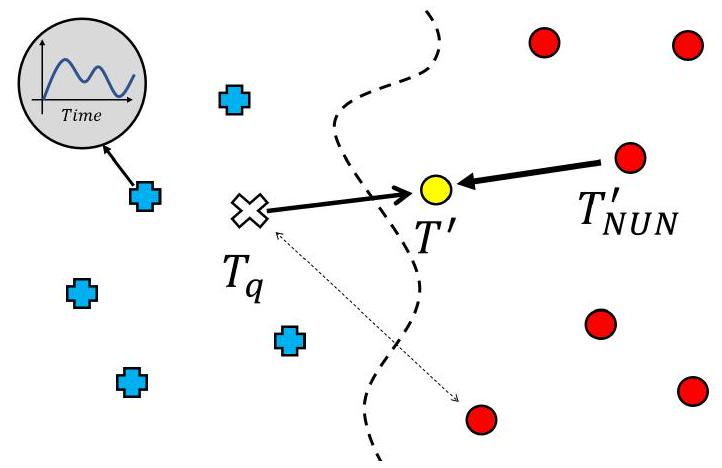
\includegraphics[width=0.4\textwidth]{CF/images/instance-based.jpg}
    \caption{A query time series $T_{q}$ (X with solid arrow) and a nearest-unlike neighbor, $T_{N U N}^{\prime}$ (red circle with solid arrow) are used to guide the generation of counterfactual $T^{\prime}$ (see yellow circle) in a binary classification task. Another in-sample counterfactual (i.e., the next NUN; other red circle with dashed arrow) could also be used to generate another counterfactual for diverse explanations.}
\end{figure}


\textbf{Step 1:} Retrieve native guide. Given a query time series, $T_{q}$, find a counterfactual instance, $T_{\text {Native }}^{\prime}$, that exists in the case-base. An example of one such instance is the query's nearest unlike neighbor $\left(T_{N U N}^{\prime}\right)$. In using these "native counterfactual" cases the method guarantees the explanation's plausibility as it is, by definition, within the distribution. However, such instances are not guaranteed to be sufficiently proximate to the query or, indeed, sparse, so an adaption step is necessary to generate the "explanatory counterfactual", $T^{\prime}$ (see Figure $3)$.

\textbf{Step 2:} Adapt native guide to generate counterfactual. To produce a more proximate explanatory counterfactual, $T^{\prime}$, the native guide, $T_{\text {Native }}^{\prime}$ is perturbed towards the to-be-explained query-case, $T_{q}$ (see Figure 3). Typically, counterfactual methods use some $L_{p}$ distance metric to guide this perturbation (such as Manhattan distance, [55]) and in time series where dynamic time warping (DTW) distance is often more appropriate an analogous averaging technique known as weighted dynamic barycentre averaging can be used 13]. In cases where we are explaining a deep-learner's predictions, the feature-weight vectors of the classifier, $\boldsymbol{\omega}$, can be used to perturb "semantically-meaningful" features of the time series, rather than the "raw" time series data, to guarantee sparsity ${ }^{4}$.
\footnotetext{Note, SHAP can also be used to generate such vectors, if we are directly explaining any given model, rather than twinning.
}

Accordingly, using the feature-weights, the method seeks to modify contiguous, subsequences, rather than the whole time series, as follows:

$$
\begin{aligned}
& T_{q}=\left\{<t_{1}, t_{2}, t_{3}, t_{4}, t_{5} \ldots, t_{n}>\right\} \text { s.t. } b\left(T_{q}\right)=c \\
& T^{\prime}=\left\{<t_{1}, t_{2}^{\prime}, t_{3}^{\prime}, t_{4}^{\prime}, t_{5} \ldots, t_{n}>\right\} \text { s.t. } b\left(T^{\prime}\right)=c^{\prime}
\end{aligned}
$$



\footnotetext{\href{https://github.com/e-delaney/Instance-Based_CFE_TSC}{https://github.com/e-delaney/Instance-Based\_CFE\_TSC}
}



%============ From TSEvo paper ============
\subsubsection{TSEvo}
We study a supervised time series classification problem. Let $x=\left[x_{1}, \ldots, x_{T}\right] \in \mathbb{R}^{N \times T}$ be a uni- or multivariate time series, where $T$ is the number of time steps and $N$ is the number of features. Let $x_{i, t}$ be the input feature $i$ at time $t$. Similarly, let $X_{:, t} \in R^{N}$ and $X_{i,:} \in R^{T}$ be the feature vector at time $t$, and the time vector for feature $i$, respectively. $Y$ denotes the output, and $f: x \rightarrow Y$ a classification model returning a probability distribution vector over classes $Y=\left[y_{1}, \ldots, y_{C}\right]$, where $C$ is the total number of classes (i.e., outputs) and $y_{i}$ the probability of $x$ belonging to class $i$. The classification model $f$ is seen as a "black-box" - i.e., no access to the inner workings of a model are available. Only the result $Y$ is observable.

\begin{definition}
Goal Properties of the TSEvo counterfactual search.
$$
\begin{aligned}
& \mathbf{R}_{\mathbf{1}}: \min \left(d\left(x, x^{c f}\right)\right), \text { s.t. } f(x) \neq f\left(x^{c f}\right) \\
& \mathbf{R}_{\mathbf{2}}: \min \left(\sum_{i=1}^{N} \sum_{t=1}^{T} \mathbbm{1}_{\left|x_{i, t}-x_{i, t}^{c f}\right| !=0}\right), \text { s.t. } f(x) \neq f\left(x^{c f}\right) \\
& \\
& \mathbf{R}_{\mathbf{3}}: x^{c f} \sim D, \text { s.t. } f(x) \neq f\left(x^{c f}\right)
\end{aligned}
$$ 
\end{definition}
The goal of counterfactual approaches is, given a time series $x$ and a classifier $f$, to provide an explanation via counter examples allowing humans to understand why classifier $f$ chose class $y$ for data point $x$ and not a counterfactual class $y^{c f}$ \cite{wachter_counterfactual_2018}. To allow such understanding, we assume that for each $x$, a counterfactual sample $x^{c f}$ can be computed, that is close to $x$, but differently classified $y \neq y^{c f}$. The resulting $x^{c f}$ is supposed to be a proximate $\left(\mathbf{R}_{1}\right)$ \cite{mothilal_explaining_2020}, sparse $\left(\mathbf{R}_{\mathbf{2}}\right)$ \cite{mothilal_explaining_2020}, and plausible $\left(\mathbf{R}_{3}\right)$ \cite{laugel_dangers_2019} adaption of $x$. Proximity refers to the distance between the query instance $x$ and the counterfactual instance $x_{c f}$, calculated as a distance measure $d$ between $x$ and $x^{c f}$. Sparsity refers to the number of feature changes between $x$ and $x_{c f}$. A plausible adaption indicates that the resulting $x^{c f}$ is in distribution with the available data $D$.

Combining the desired properties $\mathbf{R}_{1}$ and $\mathbf{R}_{\mathbf{2}}$, with a function for guiding the output distance away from the original classification leads to multi-objective problem $O$. Equation 1 shows the minimization problem. $O_{1}$ is derived from $\mathbf{R}_{1}$ by applying Mean Absolute Error as distance function $d$ \cite{mothilal_explaining_2020}, \cite{wachter_counterfactual_2018}. $O_{2}$ is consistent with $\mathbf{R}_{2}$ and $O_{3}$ denotes the output distance maximizing the output distance on a target class $l$. If no target class is chosen the second highest class probability is designated as the target.

\begin{multline}
\min O(x):=\left(O_{1}\left(x, x^{c f}\right), O_{2}\left(x, x^{c f}\right), O_{3}\left(x^{c f}\right)\right) \\
\text { s.t.f }(x) \neq f\left(x^{c f}\right) \\
O_{1}\left(x, x^{c f}\right)=\frac{1}{N * T} \sum_{i=1}^{N} \sum_{t=1}^{T}\left|x_{i, t}-x_{i, t}^{c f}\right| \\
O_{2}\left(x, x^{c f}\right)=\frac{1}{N * T} \sum_{i=1}^{N} \sum_{t=1}^{T} \mathbbm{1}_{\left|x_{i, t}-x_{i, t}^{c f}\right| \neq 0} \\
O_{3}\left(x^{c f}\right)=1-f\left(x^{c f}\right)_{l}    \\
\end{multline}

TODO : Explain how TSEvo then find the best CF

%============ From TSEvo paper ============

\subsection{Gap - From Counterfactuals for Time-Series Classification to Counterfactuals for Time-Series Extrinsic Regression} Despite advancements in counterfactual explanations for time-series classification, there exists a notable gap in extending these techniques to address extrinsic regression tasks within time-series data analysis. Bridging this gap is essential for enabling the interpretation of AI-derived insights in the context of individual health trajectories, thereby facilitating actionable recommendations tailored to individual needs.
%============ Written by ChatGPT ============


%% The Appendices part is started with the command \appendix;
%% appendix sections are then done as normal sections

% \input{table}

\newpage
\section{Methods}
Despite progress in counterfactual explanations for \gls{tsc} or \gls{tsf} \cite{theissler_explainable_2022, rojat_explainable_2021}, Table~\ref{table:xai-survey} indicates a notable gap in addressing \gls{tser} tasks. In fact, to the best of our knowledge, there currently does not exist any method for (deep learning) based explainable extrinsic regression. This work introduces novel methods for explainable \gls{tser}. 
We begin by precisely defining \gls{tser} ~(cf. Section~\ref{sec:methods:tser}). 
Afterward, we showcase our reasoning behind the choice of counterfactuals to explain \gls{tser}.
Furthermore, we outline a framework for the transformation of explainable counterfactual-based methods from classification to extrinsic regression~(cf. Section~\ref{sec:methods:tser_threshold}) and introduce definitions for desired properties for counterfactuals in \gls{tser}~(cf. Section~\ref{sec:methods:tser}) adopted from prior work~\cite{delaney_instance-based_2021}. We apply this framework to adopt four \gls{tsc} methods for \gls{tser}~(Section~\ref{sec:methods:tser_adoption}), namely 
\begin{enumerate}
    \item \gls{wachter} ~(Section~\ref{sec:methods:wachter})
    \item \gls{nunr}~(Section~\ref{sec:methods:nun})
    \item  \gls{dbar}~(Section~\ref{sec:methods:dbar})
    \item \gls{tsevor}~(~Section~\ref{sec:methods:tsevo})
\end{enumerate}
Lastly, we evaluate the four methods on the task of biological age estimation to derive recommendations for individuals to improve their health~(cf. Section~\ref{sec:methods:experiments}).


\label{sec:methods}
\subsection{\gls{tser} and User Explainability}
\label{sec:methods:tser}

\gls{tser} is a regression task that learns the mapping from time series data to a scalar value \cite{tan_time_2021}. We formally define \gls{tser} by Definition~\ref{def:tser}.
\begin{definition}
\label{def:tser}
Let $x=\left[x_{1}, \ldots, x_{T}\right] \in \mathbb{R}^{N \times T}$ be a uni- or multivariate time series, where $T$ is the number of time steps, and $N$ is the number of features. Let $x_{i,t}$ represent input feature $i$ at time $t$, and $y$ denote the output. Then, the regression model $f : x \rightarrow y$ returns an extrinsic continuous variable, with $f$ considered a "black box" — i.e., no access to the inner workings of the model is available, and only the result $y$ is observable.
\end{definition}

In Section~\ref{sec:related-work}, we discovered numerous techniques for explaining time series data. Perturbation-based, backpropagation-based, and attention-based methods have one thing in common: They show which part of the time series influences the model's output. While this is useful for the developer or a field expert, a user may not know how to interpret this explanation. When aiming for continuous health assessment, the explainability method should focus on \textit{actionability}, i.e., it should be able to show the user how to change his behavior to improve the model's output, meaning that the technique should have a local scope and target the user. Another criterion to consider is the model-specificity or model-agnosticism of an explainable technique. Indeed, as most model-specific methods focus on models used for classification, and as we explore different black-box model architectures to perform biological age estimation, we considered only post-hoc, model-agnostic methods. Model-agnostic methods allow us to explain existing models without modifying them for transparency. However, this approach does not come without drawbacks: Post-hoc methods can result in explanations based on misconceptions learned by the model rather than actual knowledge from the data \cite{laugel_dangers_2019}. From the different already implemented techniques available for \gls{tsc} (see Table \ref{table:xai-survey}), the explanation method that would provide local, user-targetted explanations while being model agnostic is called \textit{\gls{cf}}. The following subsections define how to adapt existing counterfactual methods for \gls{tsc} to \gls{tser}.
 
\subsection{Counterfactual in \gls{tser} via thresholding and its Desired Properties} 
\label{sec:methods:tser_threshold}
The common goal of counterfactual approaches is to provide an explanation via counter-examples given a time series $x$, called a query, and a model $f$. In classification scenarios, counter-examples allow users to understand why a classifier-model $f$ predicts a label $y$ for data point $x$ instead of a counterfactual class $y^{c f}$ \cite{wachter_counterfactual_2018}. However, in the case of extrinsic regression, we do not have classes as we are predicting a continuous value and not a categorical value. Using only an inequation such as $y \neq y^{c f}$  would not work since the difference between the query and the counterfactual labels could be infinitely small, providing insufficient information. Yet, we can enforce a minimal change required for a data point to be counterfactual, and this is done via thresholding: we assume that for each $x$, a counterfactual sample $x^{c f}$ can be computed that is close to $x$, but with a minimum prediction difference larger than a certain threshold $|y - y^{c f}| > \varepsilon$\footnote{\textbf{Important note:} In the specific case of biological age estimation, as we want to find a healthier patient, we are looking to decrease the \gls{ba} of the patient. Therefore, we are only interested in counterfactuals whose predicted values are lower than the patients' \gls{ba} by a certain margin (e.g., at least three years younger).}. A counterfactual should meet a few desired properties to be considered a relevant explanation for a user.
When dealing with time-series data, we typically consider the following four properties \cite{delaney_instance-based_2021}:
\begin{enumerate}
    \item Validity~(Def.~\ref{def:validity})
    \item Proximity~(Def.~\ref{def:proximity})
    \item Sparsity~(Def.~\ref{def:sparsity})
    \item Plausibility~(Def.~\ref{def:plausibility})
\end{enumerate}

Let $x=\left[x_{1}, \ldots, x_{T}\right] \in \mathbb{R}^{N \times T}$ be a uni- or multivariate time series or so-called query, where $T$ is the number of time steps, $N$ is the number of features, $x^{cf}$ a counterfactual, and $\mathcal{X}$ the input space.
Then, for a fixed $\varepsilon$, the set of valid counterfactuals denoted as $\mathcal{S}$ is defined by Definition~\ref{def:validity}.

\begin{definition}[Validity of the counterfactual]
\label{def:validity}
We define the validity property for TSER as:
$$\mathcal{S} \doteq \{x \in \mathcal{X}:\valid{x}{x^{c f}}\}$$
\end{definition}
This equation defines a set of accepted counterfactual labels for each query. It requires that the distance between the query label and the counterfactual label is larger than the threshold $\varepsilon$ but does not exceed twice the $\varepsilon$ value. The upper limit is because on the label axis, the threshold defines an area around the query where samples are not considered counterfactuals as they are too close to the query. It mimics the behavior of a class; if we move on the label axis from the query label by a distance $\varepsilon$, we are in the counterfactual area, i.e., in another class. If we move again by the same $\varepsilon$ distance, we are no longer in this counterfactual area. We are too far from the query. The latter limit is set to ensure that the  \gls{cfe} does not differ too much from the original query \cite{spooner_counterfactual_2021}.
For example, applied to biological age estimation, if we let the patient query be 56 years old and $\varepsilon = 3$, then a valid counterfactual has a label between 50 and 53 years old. A 55-year-old counterfactual is considered too close to the query to be relevant, and the lower limit ensures that a 20-year-old counterfactual is not suggested, as he would be too distant from the query.   

\begin{definition}[Proximity of the counterfactual]
We characterize the proximity property for TSER as follows:
\begin{equation}
\begin{aligned}
\min_{x^{cf}} \quad & d(x, x^{c f})\\
\mathrm{s.t.} \quad & \valid{x}{x^{c f}}\\
\end{aligned}
\end{equation}
\label{def:proximity}
\end{definition}
This property ensures that the resulting $x^{c f}$ is a proximate instance to the query \cite{mothilal_explaining_2020}. Proximity refers to the distance between the query instance $x$ and the counterfactual instance $x^{c f}$, calculated as a distance measure $d$ between $x$ and $x^{c f}$. A commonly used metric for the distance between two time series is the \gls{dtw} distance \cite{muller_dynamic_2007}.
% In the case of biological age estimation, it ensures that the query and the counterfactual have related \gls{pa} in terms of intensity.

\begin{definition}[Sparsity of the counterfactual]
We define the sparsity property for TSER as follows:
\begin{equation}
\begin{aligned}
\min_{x^{cf}} \quad & \sum_{i=1}^{N} \sum_{t=1}^{T} \mathbbm{1}_{|x_{i, t}-x_{i, t}^{c f}| \neq 0}\\
\mathrm{s.t.} \quad & \valid{x}{x^{c f}}\\
\end{aligned}
\end{equation}
\label{def:sparsity}
\end{definition}
Sparsity refers to the number of changes in data points between $x$ and $x^{c f}$ \cite{mothilal_explaining_2020}. This key property forces a \gls{cfe} method to make human-interpretable changes.
When enforcing the sparsity property, \gls{cfe} methods strive to alter the fewest variables necessary to achieve user-interpretable solutions.
Another constraint specific to time series data is that not only the fewest number of variables should change, but the changed variables should be in continuous subsequences of the original time series. Each counterfactual method implements a different technique to overcome this constraint.

\begin{definition}[Plausibility of the counterfactual]
We define the plausibility property of counterfactuals in the context of TSER as follows:
\begin{equation}
\begin{aligned}
 \quad & x^{c f} \sim D\\
\mathrm{s.t.} \quad & \valid{x}{x^{c f}}\\
\end{aligned}
\end{equation}
\label{def:plausibility}
\end{definition}
A counterfactual $x^{c f}$ is plausible if it could have been drawn from the data $D$ \cite{laugel_dangers_2019}. The plausibility property ensures that the post-hoc explanation method produces justified explanations. This property is verified by looking at the neighbors' explanation labels and analyzing whether they are close to the explanation's label. A counterfactual with a label far away from his neighbor's label is considered unjustified. In biological age estimation, a justified counterfactual has neighbors in the same age range, i.e., the distance between the counterfactual's label and the neighbor's label is below the threshold $\varepsilon$. 


\subsection{Adoption of methods for time-series extrinsic regression}
\label{sec:methods:tser_adoption}
Given our prior definitions of desired properties for counterfactuals in \gls{tser}, we describe our adoption of four methods of \acrshort{tsc} to \acrshort{tser}. Based on its results, we chose \gls{tsevo} first, as it seemed to be the more promising approach. Then we adapted Wachter, \gls{nun} and \gls{dba} to compare and put in perspective \gls{tsevo}'s results. In the following sections, we present their adoption chronologically.   

\subsubsection{\gls{wachter}-\gls{cf}}
\label{sec:methods:wachter}
The first candidate for the adoption of \gls{cfe} for \gls{tser}  is Wachter et al. \cite{wachter_counterfactual_2018} (2018). Wachter's approach involves minimizing an equation through gradient descent that combines validity~(cf.~Definition~\ref{def:validity}) and proximity~(cf.~Definition~\ref{def:proximity}) properties. To adapt Wachter's method for \gls{tser}, we replace the classifier model and introduce the threshold criterion~(cf. Section~\ref{sec:methods:tser_threshold}) while the distance function remains unchanged.
Adapting Eq. \ref{eq:wachter}~(cf. Section~\ref{sec:related-work:counterfactual_explanations}) leads to the following : 
\begin{equation} \label{eq:wachteR-cf}
\arg \min _{x^{\prime}} \max _{\lambda} \lambda\left(f_{w}\left(x_{i}\right)-\varepsilon -f_{w}\left(x^{\prime}\right)\right)^{2}+d\left(x_{i}, x^{\prime}\right)
\end{equation}
The main adaptations reside in that $f_{w}$ now denotes a black-box extrinsic regression model, and a threshold $\varepsilon$ is introduced. 

\subsubsection{\gls{nunr}-\gls{cf}}
\label{sec:methods:nun}
The second candidate for \gls{cfe} for \gls{tser} is the \gls{nun} as counterfactuals \cite{nugent_gaining_2009} (2009), and later adapted to time series data by Delaney et al.~\cite{delaney_instance-based_2021} (2021). In a classification setup, the \gls{nun} method aims to find the closest instance in the dataset that is classified differently than the query. It works by creating a reference set containing all instances in the dataset with the target classification or a different classification than the query. Then, the \gls{nun}-\gls{cf} algorithm computes the \gls{nns} of the query that are in the reference set, obtaining the \gls{nuns}. The \gls{nns} are computed using $KNeighborsTimeSeries$ \cite{tavenard_tslearn_2020}.
We must only modify how the reference set is defined to adapt the \gls{nun}-\gls{cf} algorithm to the regression setup.
\begin{definition}[Reference set]
    \label{def:ref-set}
    % \textbf{Reference set} \\
    The reference set is a subset of all known data $D$ with a valid prediction under def. \ref{def:validity}.
    \[
        R = \{z \in D : \valid{x}{z}\}
    \]
\end{definition}
With \gls{nunr}-\gls{cf}, if a \gls{nun} exists, it is guaranteed that the found counterfactual is in the data distribution, as it is an existing sample~(cf.~Def.~\ref{def:plausibility}) and valid~(cf.~Def.~\ref{def:validity}). The proximity~(cf.~Def.~\ref{def:proximity}) of the counterfactuals will be minimized among the existing valid samples, but as shown in previous work \cite{delaney_instance-based_2021, hagen_dice_2020}, the \gls{nun} is not necessarily close to the model decision boundary, and it is possible to find more proximate counterfactuals by mutating the \gls{nun} towards the decision boundary. These mutations are typically done by perturbing the query time series on areas where the query and the \gls{nun} disagree. Another issue is that \gls{nuns} are not sparse; in the context of biological age estimation, the \gls{nunr}-\gls{cf} algorithm locates a physical activity that closely resembles the query's physical activity but is performed by a different individual and slightly varies at each timestamp.

\subsubsection{\gls{dbar}-\gls{cf}}
\label{sec:methods:dbar}
The third method we consider is called \gls{dba}-\gls{cf} and was proposed by Delaney et al. \cite{delaney_instance-based_2021} in 2021. The main idea is to bring the found \gls{nun} closer to the decision boundary by averaging between the query and the \gls{nun}. Originally, Forestier et al. \cite{forestier_generating_2017} (2017) proposed \gls{dba} to augment time-series datasets. \gls{dba} is used to compute the average between time series. The concept behind \gls{dba}-\gls{cf} is to achieve a weighted average between the query and the \gls{nun}, starting with all the weight on the query and then iteratively moving the weight towards the \gls{nun} until the decision boundary is reached.
\subsubsection{\gls{tsevor}-\gls{cf}}
\label{sec:methods:tsevo}
\gls{tsevo} is a technique that combines time series perturbation approaches from the recent work\cite{guilleme_agnostic_2019} and \cite{mujkanovic_timexplain_2023} with a genetic algorithm for multi-objective optimization \cite{dandl_multi-objective_2020}. This technique allows the creation of model-agnostic counterfactual explanations for uni- and multivariate classification problems.
% Unlike previous techniques described in \cite{delaney_instance-based_2021}, \cite{guilleme_agnostic_2019}, and \cite{mujkanovic_timexplain_2023}, \gls{tsevo} does not require an advanced decision regarding the transformer to be made.

\gls{tsevo} tackles the challenge of finding a counterfactual that meets the four key properties validity \ref{def:validity}, proximity \ref{def:proximity}, sparsity \ref{def:sparsity} and plausibility \ref{def:plausibility}. To achieve this, \gls{tsevo} treats each property as an objective to optimize, forming a multi-objective optimization problem. We define below how the properties are transformed into objectives in the setting of \gls{tser}. 

\begin{definition}[Multi-Objective Problem]
$O_{1}$ is derived from def. \ref{def:proximity} by applying \gls{mae} as distance function $d$ \cite{mothilal_explaining_2020}, \cite{wachter_counterfactual_2018}.
$$O_{1}(x, x^{c f})=\frac{1}{NT} \sum_{i=1}^{N} \sum_{t=1}^{T}|x_{i, t}-x_{i, t}^{c f}|$$ $O_{2}$ is consistent with def. \ref{def:sparsity}.
$$O_{2}(x, x^{c f})=\frac{1}{NT} \sum_{i=1}^{N} \sum_{t=1}^{T} \mathbbm{1}_{|x_{i, t}-x_{i, t}^{c f}| \neq 0}$$ $O_{3}$ denotes the normalized output distance.
$$O_{3}(x, x^{c f})=(f(x) - f(x^{c f})-\varepsilon) / \varepsilon$$ Combining the desired properties leads to the following multi-objective problem $O$:
\begin{equation}
\begin{aligned}
\min_{x^{cf}} \quad & O(x, x^{cf}):=(O_{1}(x, x^{c f}), O_{2}(x, x^{c f}), O_{3}(x^{c f}))^T\\
\mathrm{s.t.} \quad & \valid{x}{x^{c f}}\\
\end{aligned}
\end{equation}
\end{definition}
The multi-objective optimization follows the steps described in the original \gls{tsevo} publication \cite{hollig_tsevo_2022}.
In summary, a population of $n$ individuals is initialized, where each individual represents a potential counterfactual.
The individuals are evaluated with respect to their objectives score.
For $g$ generations, the evolution algorithm selects the best individuals in the population according to how they fulfill the different objectives. Depending on a certain probability, it performs crossover and/or mutates them. For the mutations, we used the authentic opposing information mutation, first introduced by Guilleme et al. \cite{guilleme_agnostic_2019}, which is based on the assumption that interpretable values of time series can exhibit shapes (e.g., peaks) that are easily understandable to humans.
To use those shapes included in a reference set $R$~(cf.~Def.~\ref{def:ref-set}), we draw a random sample $r \in R$. 
Both $r$ and the selected individual $\lambda_i$ are segmented with window size $w_i$, resulting in $S(r)$ and $S(\lambda_i)$. The mutation then draws a random segment index $s \in [ 0,|S(r)|-1]$ and replaces the drawn slice $S(\lambda_i)[s]$ with the slice $S(r)[s]$ from the replacement time series. The concept of crossover in genetic algorithms is utilizing the search space by merging the genetic material of high-performing individuals \cite{mitchell_introduction_1998}.
The reference set is used in the evolution algorithm to mutate the individuals. It ensures that the mutated individuals stay in the data manifold. Note that this is meant to achieve the plausibility property~(cf.~Def.~\ref{def:plausibility}) by design, as this property was not expressed as an objective.

\subsection{Experimental Evaluation}
\label{sec:methods:experiments}
Our work was motivated by the findings of Pyrkov et al. \cite{pyrkov_extracting_2018} and Rahman et al. \cite{rahman_deep_2019}, who showed that deep learning models could estimate the biological age of a patient from his physical activity. Once we predict the biological age, we can use counterfactual explanations to give feedback to the patient.

The following Sections describe our efforts to reproduce prior work to train models for biological age estimation, enabling us to test our \acrshort{cfe} methods. For the training and data generation, we followed the same steps as described in prior work in Pyrkov et al. \cite{pyrkov_extracting_2018}, Rahman et al. \cite{rahman_deep_2019}, and Shim et al. \cite{shim_wearable-based_2023}. Figure \ref{fig:pipeline} shows an overview of the whole pipeline, from data generation to providing recommendations.

\begin{figure}
    \centering
    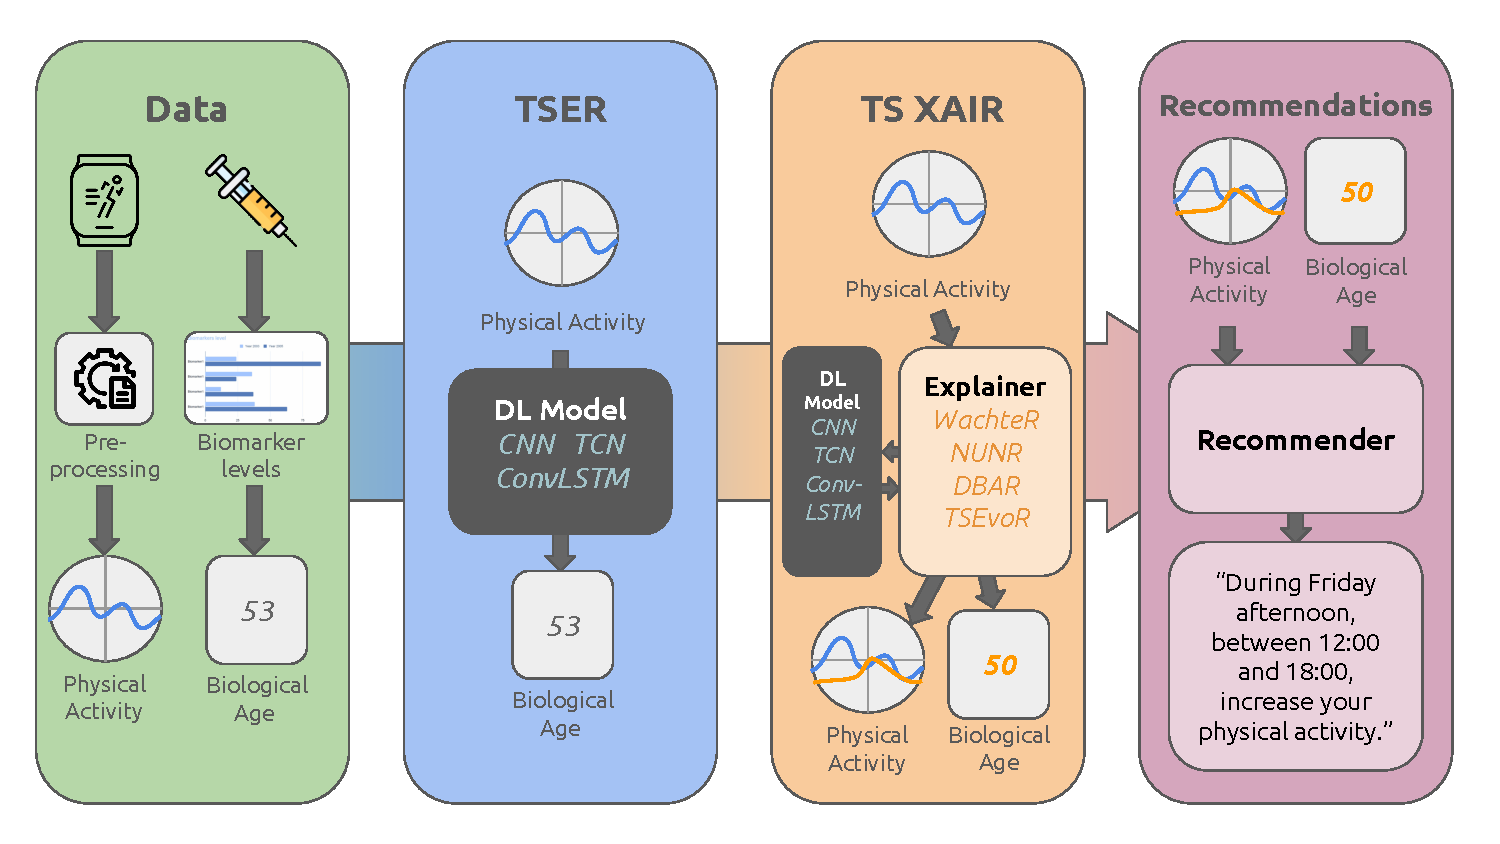
\includegraphics[width=1\linewidth]{images/pipeline.pdf}
    \caption{Pipeline: From data preprocessing to physical activity recommendations.}
    \label{fig:pipeline}
\end{figure}

\subsubsection{Physical Activity}
\textbf{Description} We used physical activity data recorded during the \gls{nhanes} from 2003 to 2004 \cite{cdc_nhanes_2003} and from 2005 to 2006 \cite{cdc_nhanes_2005}. 
\gls{nhanes} uses a complex sampling design to survey non-institutionalized members of the US population.
A subset of \gls{nhanes} participants recorded their activity data. During the survey, participants' physical activity is tracked for seven continuous days using a physical activity monitor\footnote{The monitor used was the ActiGraph AM-7164; ActiGraph, Pensacola, FL, USA} to record \textit{activity counts} sampled every minute. 
The participants wear the monitors on the right hip using an elastic belt.
The datasets included 14'631 participants, with 7'176 in 2003-2004 and 7'455 in 2005-2006.
\textbf{Filtering} The filtering steps are based on prior work done on biological age estimation~\cite{pyrkov_extracting_2018, rahman_deep_2019, shim_wearable-based_2023}. First, we removed outliers with abnormally low ($< 50$) or high ($>5000$) mean activity count. Then, we removed patients with less than 10'080 ($= 7 \times 24 \times 60$) activity counts, corresponding to one measurement every minute for seven days. Also, we only considered days where the participant was active for more than 200 minutes. Therefore, we filtered out participants who had less than four days of meeting this criteria. This filter resulted in a total of 9,591 individuals.
\textbf{Transformation} To handle the noisy and outlier-filled nature of the time-series human locomotor data, we first needed to apply some basic data transformation operations, such as smoothing.
The physical activity intensity $(pa_{intensity})$ values range over a large magnitude and are always positive, so we applied log transformations to the data, as suggested by Rahman et al. \cite{rahman_deep_2019}.
However, since the original data contains some $0$ values, we added a negligible value ($1$) before applying log transformations.
The first transformation is a Box-Cox \cite{box_analysis_1964} transformation with $\lambda = 1$, which is equivalent to a simple log transformation (other values of $\lambda$ were investigated by Rahman et al. \cite{rahman_deep_2019}).
Then, a second log transformation is computed. Since the data is a sequential time series of seven days, we applied moving averages on the data with different window sizes and an \gls{ema}. 
\begin{equation}
    pa_{log} = \log(BoxCox(pa_{intensity} + 1) + 1)
\end{equation}
\begin{equation}
    pa_{ema}^i = 
    \begin{cases}
      pa_{log_i}, & \mathrm{if}\ i=1 \\
      \alpha pa_{log_i} + (1 - \alpha) pa_{log_{i-1}}, & \mathrm{otherwise}
    \end{cases}
\end{equation}

We used $\alpha = \frac{1}{N+1}$ and $N=35$, as it was reported to be the best window size by Rahman et al. \cite{rahman_deep_2019}.

\subsubsection{Biological Age}
We used the \gls{nhanes} 2003-2006 anthropometric and bio-marker datasets to compute each patient's biological age \cite{kwon_toolkit_2021}.
The biomarker dataset contained information on albumin, alkaline phosphatase, blood urea nitrogen, uric acid, cholesterol, creatinine~\cite{cdc_biopro_d_2005}, C-reactive protein~\cite{cdc_crp_d_2005}, body mass index~\cite{cdc_bmx_c_2003}, glycohemoglobin~\cite{cdc_l10_c_2003}, systolic and diastolic blood pressure~\cite{cdc_bpq_c_2003}, lymphocyte percentage, mean cell volume and white blood cell count~\cite{cdc_l25_c_2003}.
% BIOPRO_D
% albumin
% alp =  Alkaline Phosphatase
% bun =  blood urea nitrogen
% uap =  uric acid
% totchol = Cholesterol
% lncreat = Creatinine (mg/dL) 
% 
% CRP_D
% crp = C-reactive protein
% 
% BMX_C
% bmi = Body Mass Index
% 
% L10_C
% hba1c = Glycohemoglobin 
% 
% BPQ_C
% sbp = Systolic and diastolic blood pressure
% 
% L25_C
% lymph = Lymphocyte percent
% mcv = Mean cell volume
% WBC = White blood cell count
Then, we used the Klemera-Doubal method \cite{klemera_new_2006} to compute a mapping between the biomarkers information and the biological age. We retained only patients aged between 18 and 85. As a result, we obtained a dataset of 10,184 patients along with their corresponding biological age.
Lastly, we combined the physical activity dataset with the biological age datasets, resulting in 7'222 matched patients. Not all patients in the physical activity dataset were included in the biomarker dataset, hence the lower total number of patients. We split the combined dataset into training ($65\%$), validation ($25\%$), and testing ($10\%$) sets, yielding 4'694, 1'805 and 723 patients, respectively.
\subsubsection{Deep Learning models for Biological Age Estimation}
Using physical activity data to predict biological age is an example of a \gls{tser} task. In our scenario, we trained and tested three different models to predict biological age from physical activity data: 

\begin{enumerate}
    \item A \textit{\gls{cnn}} suggested by Pyrkov et al. for biological age estimation \cite{pyrkov_extracting_2018}
    \item A \textit{\gls{convlstm}} proposed by Rahman et al. for biological age estimation \cite{rahman_deep_2019}.
    \item A \textit{\gls{tcn}} \cite{lea_temporal_2016, bai_empirical_2018} network. 
    \end{enumerate}
To the best of our knowledge, the \gls{tcn} model has not yet been tested for biological age estimation in prior work. It was included in the evaluation in this work because recent literature indicates that \gls{tcn} models can achieve state-of-the-art results on time series tasks while often being less complex than \gls{lstm} models~\cite{bai_empirical_2018}.
Each model requires a different data representation: The \gls{cnn} takes as input a flat vector of 10'080 values, \gls{convlstm} uses a complex 3D representation ($60, 24, 7$), and \gls{tcn} falls in between the two, taking vectors of shape $(7, 1440)$, where the days are treated as features. We trained all models on the training data for \gls{convlstm} and \gls{cnn}; we used the steps and hyperparameters described by Rahman et al.~\cite{rahman_deep_2019} and Pyrkov et al.~\cite{pyrkov_extracting_2018} respectively.
                 % num_channels: list[int] = [128]*10,
                 % kernel_size: int = 4,
                 % dropout: float = 0.2,
                 % num_timestamps: int = PhysicalActivity.NumberOfMinutesPerDay,
                 % patience: int = 10,
                 % verbose: bool = False,
                 % delta: int = 0,
                 % % save_model: bool = True):
The \gls{tcn} has ten layers of 128 channels each; we used a kernel size of 4 and a dropout of 0.2. We trained the model for 100 epochs, with a learning rate 0.0001, and we chose the best model according to the \gls{mse} loss. We recorded two other metrics, which are the \gls{mae}, which gives a more intuitive comprehension of the error of the model than the \gls{mse}, and the Pearson correlation, which indicates the strength of the linear association between the physical activity and the biological age. 

\subsubsection{Explainable Biological Age Estimation}
Utilizing our counterfactual adaptations \gls{wachter}, \gls{nunr}, \gls{dbar} and \gls{tsevor}, we generated counterfactuals with threshold $\varepsilon=3$~(cf.~Section~\ref{sec:methods:tser_threshold}) for each sample of the 723 samples in the test set using the three different models.
For \gls{wachter}, we defined a loss function from eq. \ref{eq:wachteR-cf}:
\begin{equation}
    \label{eq:wachter-loss}
    \text{LOSS} = \lambda\left(f_{w}\left(x_{i}\right)-\varepsilon -f_{w}\left(x^{\prime}\right)\right)^{2}+\left(1-\lambda\right)d\left(x_{i}, x^{\prime}\right)
\end{equation}
and $x^{\prime}$ was initialised  to $x_{i}$ (we also attempted random initialization). 
Using the L1-Norm as distance function $d$, we then performed a gradient descent using the ADAM \cite{kingma_adam_2017} optimizer for $n=100$ iterations for each lambda $\lambda$ and increased lambda by $0.05$ if no valid (Def. \ref{def:validity}) counterfactual is found. The valid counterfactual with the smallest loss~(Eq.~\ref{eq:wachter-loss}) is returned. If no valid counterfactual is found after trying out all lambdas, we return the counterfactual with the smallest corresponding loss.
For \gls{nunr}, once the reference set is adapted (see \ref{def:ref-set}), the remainder of the algorithm is the same as in a classification setting.
For \gls{dbar}, we retrieved the \gls{nun} and performed a weighted sum: 
\begin{equation}
    x^{cf} = DBA(\beta x_{query}, (1-\beta)x_{NUN})
\end{equation}
We chose to run $10$ iterations, increasing $\beta$ by $0.01$ at each iteration and returning $x^{cf}$ as soon as it is valid. 
For \gls{tsevor}, we used the genetic algorithm over 50 generations and applied mutation to the individuals using the authentic opposing information transformer, as implemented by Guillemé et al. \cite{guilleme_agnostic_2019}.

\subsubsection{Habits recommendations}
The generated counterfactuals depict time series plots of recommended physical activity data. Presenting this data to potential patients allows them to interpret what actions they should take to improve their biological age. However, different patients might interpret the counterfactuals differently. 
We designed a system that provides the patient with highly interpretable text feedback to give a more concrete, text-based recommendation. This feedback contains a few sentences or \textit{recommendations} on how to adjust the activity based on the generated counterfactuals. Each day is separated into four parts of six hours each to generate a recommendation $R$:
\begin{center}
    \textit{Night, Morning, Afternoon,} and \textit{Evening}.
\end{center}
For each part $p$, we compute the mean value of the query's physical activity $mean_q$ and the mean of the counterfactual's physical activity $mean_{cf}$. We assume that the obtained means represent a percentage activity on a scale from \textit{No Intensity $(0\%)$} to \textit{Very High Intensity $(100\%)$}. This representation allows us to interpret the difference between $mean_q$ and $mean_{cf}$ as a 
 percentage change. Concretely, this percentage change ($Percentage_{change}$) is defined as follows, where MAX ACTIVITY INTENSITY denotes the maximum value of the intensity of the counterfactual and the query.

% One issue to take into account is that if the query mean is close to zero, for example, 0.1, and the counterfactual mean is, for example, 2, then the change percentage is $ \frac{2 - 0.1}{0.1} * 100 \eq 1900\%$ which is not very intuitive
\begin{equation}
    Percentage_{change} = \frac{mean_{cf} - mean_{q}}{\text{MAX ACTIVITY INTENSITY}} \times 100
\end{equation}
Using our approach, we generate several maximum $n$ recommendations to the user and only include recommendations suggesting a minimal percentage change of at least $p$\%, with $n$ and $p$ being configurable parameters.
\newpage

% \subsubsection{Qualitative Evaluation with Social Science}
% Spreitzer et Al. \cite{spreitzer_evaluating_2022} (2022) examined the practicality of counterfactual explanations (CEs) for end users based on five social science criteria. 
% \begin{itemize}
% \item \textbf{Contrastiveness}: People focus on understanding why a specific event occurred instead of another possible outcome. Regarding counterfactual explanations, contrastiveness is based on how well the user comprehends what changes are necessary to achieve the opposite result.
% \item \textbf{Selectivity}: Generally, humans are not accustomed to seeking a complete cause for an event. Rather, we tend to identify a smaller set of causes and consider them a complete explanation. Therefore, counterfactual explanations can help offer a more selective approach by altering only a subset of features and suggesting alternative possibilities.
% \item \textbf{Social}: Explaining information to a user is a two-way interaction between the user and the system. Therefore, it's important to consider the social environment, target audience, and specific use cases when explaining. Any proposed changes should be realistic and applicable to the affected person's situation regarding counterfactual explanations.
% \item \textbf{Truthful}: A clear explanation must be perceived as plausible.
% \item \textbf{Consistent with prior beliefs}:  End-users are more likely to consider counterfactual explanations that suggest changes expected in advance due to their tendency to ignore information inconsistent with their prior beliefs. 
% \end{itemize}

% We use these criteria as an evaluation grid for the counterfactual plots~(cf.~Fig.~\ref{fig:quali-eval}).

\section{Results}
\label{sec:results}
To evaluate the performance of the counterfactuals, we use the same metrics as Höllig \& Al. \cite{hollig_tsevo_2022}.

Validity
Plausibility
Sparsity
Number of data points changed

\section{Discussion}
\label{sec:discussion}


Our work aims to introduce novel methods for explainable time series extrinsic regression for \gls{xai} applications. Our interest was primarily focused on model-agnostic user-targeted explanations. To achieve this, we have adapted four counterfactual techniques from the domain of time series classification. We outline principal findings, practical implications, limitations below and also provide a comparison with prior work.



\subsection{Principal findings}
% Summary: A brief recap of your key results
% aim for a clear statement of the overall result that directly answers your main research question. This should be no more than one paragraph.
% More specifically, we strongly believe that shifting the paradigm of reactive healthcare to preventive healthcare is essential to break the rising costs of health, and this can be done effectively by combining the recent boom of wearable sensors and novel AI solutions. 
The plots~(see~Fig.~\ref{fig:quali-eval}) illustrate how the evolution of techniques from left to right affects the quality of generated counterfactuals. \gls{wachter} technique utilizes noise to produce a counterfactual, but it mostly fails due to an excessive emphasis on the proximity metric. \gls{nunr}, which finds an existing counterfactual instance, is advantageous because it is highly plausible since it is based on someone else's activity. However, it suggests a lot of different changes and lacks sparsity. \gls{dbar} is an improvement on \gls{nunr}, using an average between the query and NUN to improve the proximity metric, but at the cost of validity and plausibility, without addressing the sparsity issue. \gls{tsevor} uses powerful time series transformers to mutate subsequences of existing instances, resulting in sparse, proximate, plausible, and valid counterfactuals. 
Looking at the numbers, the fact that \gls{nunr} has only around $50\%$ of plausibility indicates the counterfactual, which is an instance of the dataset in the \gls{nunr} case, has a label close to only half its neighbors. This indicates a noisy model that predicts differently close instances. When using a \gls{tcn} or a \gls{cnn}, \gls{tsevor} manages to find a valid counterfactual in $40\%$ of the cases. This percentage drops when \gls{tsevor} is used with the \gls{convlstm} because of its use of a complex data representation. 
We can see that \gls{tsevor} is the only technique that manages to find proximate, sparse, and highly plausible counterfactuals.
The \gls{tsevor}-generated counterfactual explanations are easy to understand at a glance, delivering high-quality feedback to users.

\subsection{Comparison with prior work} 
 Previous research has tackled similar tasks in the field. Perturbation techniques such as DynaMask \cite{crabbe_explaining_2021} can be used to highlight essential subsets of time series data. While it is useful for exp
 laining \gls{tser}, it does not focus on the user. Counterfactual techniques have been developed for \gls{tsc} \cite{hollig_tsevo_2022, delaney_instance-based_2021} and \gls{tsf} \cite{wang_counterfactual_2023} tasks. However, these techniques require some modifications to explain \gls{tser} tasks. As far as we know, no explainable technique specifically targeting users for \gls{tser} models exists.

\subsection{Practical implications}
Our algorithms can be used to explain any univariate \gls{tser} task, we did not test it on multivariate data. For biological age estimation, our work brings the final piece of the puzzle for continuous health assessments using wearable devices. Using Counterfactual explanation, a smartphone app provides meaningful feedback on how the patient should modify his physical activity to improve his health. Our research on biological age estimation is not limited to that particular area, as our approach can be applied to any \gls{dl} technique that aims to learn a score from time series data. For instance, it can be used to understand how the mortality rate of people affected by contagious disease would change depending on the variation of the number of contagions, as indicated in Diaz-Lozano et al.'s study on COVID-19 \cite{diaz-lozano_covid-19_2022}. Similarly, our approach can demonstrate the impact of the hourly total number of parked cars on the daily occupancy rate, as shown in Stolfi et al.'s study \cite{stolfi_predicting_2017}. If a task related to \gls{tser} is being performed and a \gls{dl} model is showing good results, we can use our new \gls{tsevor} approach to identify counterfactuals. The capacity of \gls{tsevor} to find valid counterfactuals (as defined in Definition \ref{def:validity}) is dependent on the reference set's size (as defined in Section \ref{def:ref-set}). The number of mutations that \gls{tsevor} can attempt is determined by the size of the reference set, and if the reference set is empty, it will not be able to identify any counterfactuals. The plausibility of the counterfactuals may vary depending on the accuracy of the \gls{dl} model (as explained in Section \ref{def:plausibility}). Currently, our best methods have achieved 60\% plausibility, indicating that there is still room for improvement.
% Our work bring  brings the final piece of the puzzle for continuous health assessments using wearable devices.
% \begin{enumerate}
%     \item The patient continuously collects physical activity using a wearable device, such as a smartwatch.
%     \item A trained deep-learning model predicts biological age, an indicator of the patient's current health status.
% \end{enumerate}
% Interpretations: What do your results mean?
% Implications: Why do your results matter?
% \subsection{Comparison with prior work}
% No available before.

\subsection{Limitations}
In order to improve our approach, it's important to acknowledge some limitations that are inherent in our implementation and methodology. First, the computation times for \gls{tsevor} are quite long, which suggests that we could benefit from using parallelization strategies to speed up the process. Second, our reliance on specific models like \gls{tcn}, \gls{cnn}, and \gls{convlstm} can lead to variable results, which raises questions about the fairness of comparisons and the need for more robust models \cite{hamman_robust_2024} with lower \gls{mae}. Third, the selection of thresholds is somewhat arbitrary and can have unexplored implications for the outcomes \cite{spooner_counterfactual_2021}. In addition, our algorithms have primarily been tested on univariate time-series data, which could limit their applicability to more complex datasets. Finally, the effectiveness of \gls{tsevor} depends heavily on the availability of a valid reference set, which means it may not be effective in scenarios where such data is lacking. Therefore, it's important to explore alternative strategies in those cases. By addressing these limitations, we can develop a more comprehensive and reliable framework for generating counterfactuals.
% Limitations: What can’t your results tell us?
% Here, just mention one paragraph about general limitations of our implementation and approach. The following things come to mind spontaneously:
% \begin{enumerate}
%     \item Computation times -> \gls{tsevo} is slow -> could be improved by parallelization
%     \item Our results highly depend on the model (\gls{tcn}, \gls{cnn}, \gls{convlstm}) and their performance (is it fair to compare a 14.85 MAE \gls{tcn} with a 17.35 MAE \gls{tcn}?) -> In the future there might be models with a lower MAE and hence should be used to generate more robust counterfactuals; there are also metrics to measure robustness of counterfactuals across different models: https://arxiv.org/abs/2305.11997
%     \item The choice of the threshold is somewhat arbitrary, we did not study its effects.
%     \item Algorithms were only tested on univariate time-series
%     \item \gls{tsevor} highly depends on the reference set~(cf.~Def.~\ref{def:ref-set}), which means that if there is no valid \gls{nun} in the dataset, the method will not be able to produce any counterfactual. 
% \end{enumerate}

%\subsubsection{\gls{wachter}}
%One advantage of \gls{wachter} is that it does not require access to any other sample in the dataset to generate a counterfactual explanation, which is not the case for \gls{nunr}, \gls{dbar} and \gls{tsevor}, which need a reference set~(cf.~Def.~\ref{def:ref-set}). As this method only constraints counterfactuals on their validity \ref{def:validity} and proximity \ref{def:proximity}, it fails to produce sparse \ref{def:sparsity} counterfactuals. Another point is that choosing the right value for lambda is difficult; we were not able to find a suitable parameter that would produce consistently proximate \textit{and} valid counterfactuals.

%\subsection{Native Guide}
%To mutate the \gls{nun} towards the decision boundary, we first aimed to adapt the Native Guide methods \cite{delaney_instance-based_2021}. Native Guide guides the \gls{nun} by using the last layer of the classification model. With the help of GradCAM \cite{selvaraju_grad-cam_2020}, it finds the discriminative part of the query and modifies it using the found \gls{nun} to find a proximate counterfactual. The adaptation of GradCAM for the regression case was not further investigated and remains open for future research.

%\subsubsection{Setting thresholds for regression models is brittle ?}
%Spooner \& Al. \cite{spooner_counterfactual_2021} argue that the choice of the threshold has an influence on the found counterfactual. The authors discuss using thresholds to specify the validity of counterfactuals (CFs) for scalar regression problems, as we did in this work. They claim that it can result in unrealistic CFs far from the query point when the distance in x exceeds the threshold value. Their article proposes a potential-based search approach, assigning a scalar potential to each output y, quantifying the value associated with candidate counterfactual points. This approach formalizes the notion of regression counterfactuals in terms of potentials instead of thresholds, which can lead to more accurate results. We believe that we resolved the unrealistic issue by providing an outer limit for the counterfactual label; it would be interesting to compare the potential approach, but we decided not to because of the code's unavailability.



\section{Outlook}
\label{sec:outlook}
Some Outlook


%% The Appendices part is started with the command \appendix;
%% appendix sections are then done as normal sections
\appendix

\section{Sample Appendix Section}
\label{sec:sample:appendix}
Lorem ipsum dolor sit amet, consectetur adipiscing elit, sed do eiusmod tempor section \ref{sec:sample1} incididunt ut labore et dolore magna aliqua. Ut enim ad minim veniam, quis nostrud exercitation ullamco laboris nisi ut aliquip ex ea commodo consequat. Duis aute irure dolor in reprehenderit in voluptate velit esse cillum dolore eu fugiat nulla pariatur. Excepteur sint occaecat cupidatat non proident, sunt in culpa qui officia deserunt mollit anim id est laborum.

%% If you have bibdatabase file and want bibtex to generate the
%% bibitems, please use
%%
\newpage
\newpage
\bibliographystyle{elsarticle-harv} 
\bibliography{references}

%% else use the following coding to input the bibitems directly in the
%% TeX file.

% \begin{thebibliography}{00}

% %% \bibitem[Author(year)]{label}
% %% Text of bibliographic item

% \bibitem[ ()]{}
\clearpage

\printglossaries
% \end{thebibliography}
\end{document}

\endinput
%%
%% End of file `elsarticle-template-harv.tex'.
